\documentclass[aps,prd,twocolumn,showpacs,superscriptaddress,nofootinbib]{revtex4-2}

\usepackage{amsmath,amssymb}
\usepackage{graphicx}
\usepackage{booktabs}
\usepackage{siunitx}
\usepackage{hyperref}

\begin{document}

\title{Analog Hawking Radiation in the Graphene Dirac Fluid:\\
Predictions from Schwinger-Keldysh Dissipative EFT}

\author{SK-EFT Hawking Research Program}

\date{\today}

\begin{abstract}
We adapt the Schwinger-Keldysh dissipative effective field theory (SK-EFT)
framework to predict analog Hawking radiation in graphene Dirac fluid flow.
The graphene Dirac fluid near the charge neutrality point is a natively
relativistic 2+1D system with sound speed $c_s = v_F/\sqrt{2} \approx
\SI{710}{\kilo\meter/\second}$ (monolayer) set by the conformal equation
of state $\varepsilon = 2p$. A sonic horizon forms where the drift velocity
reaches~$c_s$---a condition already achieved by the Dean group at Columbia
(Geurs~\textit{et~al.}, 2025) in a bilayer graphene de~Laval nozzle.

For the Dean bilayer nozzle, we predict $T_H \approx \SI{2.4}{\kelvin}$
(nine orders of magnitude above BEC), with a well-controlled EFT expansion
(adiabaticity $D = 0.23$, dispersive correction $\delta_{\rm disp} = -2.8\%$).
The dissipative correction $\delta_{\rm diss} \sim 10^{-13}$ is negligible---11
orders of magnitude below the dispersive correction---because the viscous
damping rate $\Gamma_H \approx \SI{0.3}{\per\second}$ is vastly smaller
than the surface gravity $\kappa \sim \SI{e12}{\per\second}$. The Hawking
signal manifests as excess current noise $\Delta S_I \approx
\SI{e-26}{\ampere\squared/\hertz}$ across a \SIrange{0.5}{85}{\giga\hertz}
band---roughly 1\% of the thermal Johnson-Nyquist background---extractable
via broadband correlation analysis. The corrected noise formula
$\Delta S_I(\omega) = 2\hbar\omega\,\sigma_Q\,\Gamma(\omega)\,n_H(\omega)$,
derived independently from Keldysh FDT and Landauer-B\"uttiker with
Bogoliubov mixing, gives statistical integration times under one second
for $5\sigma$ discovery (greybody $\Gamma \geq 0.01$), making the
measurement systematics-limited rather than statistics-limited.

We classify transport coefficients for the 2+1D charged conformal fluid:
2~independent first-order coefficients ($\eta$, $\sigma_Q$) matching the
1+1D BEC count, but ${\sim}9$ at second order (vs.\ 2~in BEC), reflecting
the richer tensor structure of 2+1D. The giant Wiedemann-Franz violation
($L/L_0 > 200\times$, Majumdar~\textit{et~al.}, 2025) arises from two-channel
transport: charge ($\sigma_Q$) and heat ($\kappa_{\rm th} \propto s^2/\sigma_Q$),
consistent with the SK-EFT two-channel structure. All predictions are
formally verified in Lean~4 (32~theorems, zero sorry) and derive from
a computation pipeline with 99~tests.
\end{abstract}

\maketitle

%% ================================================================
\section{Introduction}
\label{sec:intro}

Analog gravity---the study of effective curved spacetimes in condensed matter
systems---has matured from a theoretical proposal~\cite{Unruh1981} to an
experimental science. Steinhauer's observation of thermal Hawking radiation
at $T_H \approx \SI{0.35}{\nano\kelvin}$ in a $^{87}$Rb Bose-Einstein
condensate (BEC)~\cite{deNova2019} confirmed the Planckian spectrum predicted
by Hawking, while polariton superfluids have demonstrated negative-energy
waves~\cite{Falque2025}. These systems share a common theoretical
infrastructure: the acoustic metric theorem of Unruh~\cite{Unruh1981} and
Visser~\cite{Visser1998}, which maps phonon propagation in a moving fluid to
massless scalar fields on a curved background.

The Schwinger-Keldysh (SK) effective field theory framework of
Crossley, Glorioso, and Liu~\cite{CGL2017a,CGL2017b} provides a systematic
derivative expansion for dissipative corrections to the acoustic Hawking
temperature. Papers~1--4 of this series applied this framework to 1+1D BEC
phonon hydrodynamics, establishing: (i)~a transport coefficient counting
formula ${\rm count}(N) = \lfloor(N{+}1)/2\rfloor + 1$; (ii)~CGL
fluctuation-dissipation relations (FDR) constraining noise from dissipation;
(iii)~an exact WKB connection formula for the Hawking spectrum with
dispersive and dissipative corrections; and (iv)~formal verification of all
results in Lean~4.

In this paper, we extend the SK-EFT framework to the \emph{graphene Dirac
fluid}---a natively relativistic 2+1D system where electron-hole
quasiparticles propagate at the Fermi velocity $v_F \approx
\SI{e6}{\meter/\second}$. Three recent experimental developments motivate
this extension:
\begin{enumerate}
\item Geurs~\textit{et~al.}~\cite{Geurs2025} demonstrated \emph{supersonic
electron flow} through a de~Laval nozzle in bilayer graphene, creating the
first electronic sonic horizon ($v > c_s \approx \SI{440}{\kilo\meter/\second}$).
\item Majumdar~\textit{et~al.}~\cite{Majumdar2025} measured universal quantum
critical transport at the Dirac point: $\sigma_Q \approx 4\,e^2/h$, a
Wiedemann-Franz violation exceeding $200\times$, and $\eta/s$ within a factor
of~4 of the Kovtun-Son-Starinets (KSS) bound~\cite{KSS2005}.
\item Zhao~\textit{et~al.}~\cite{Zhao2023} directly measured the electronic
sound speed $c_s = v_F/\sqrt{2}$, confirming the conformal equation of state.
\end{enumerate}

The predicted Hawking temperature for the Dean nozzle, $T_H \approx
\SI{2.4}{\kelvin}$, is \emph{nine orders of magnitude} larger than in BEC.
Moreover, graphene's dispersion corrections are \emph{subluminal} (many-body
Coulomb renormalization makes $v_F(k)$ increase at small~$k$), unlike BEC's
superluminal Bogoliubov dispersion. This makes the Hawking temperature formula
\emph{more robust}: high-momentum modes propagate slower than low-momentum
modes and cannot escape the horizon, eliminating the trans-Planckian
complications of BEC.

%% ================================================================
\section{Acoustic Metric for the Dirac Fluid}
\label{sec:metric}

\subsection{Conformal equation of state}

The graphene Dirac fluid near the charge neutrality point (CNP) is described
by relativistic hydrodynamics with the conformal equation of state
$\varepsilon = 2p$ (tracelessness of $T^\mu{}_\mu$ in 2+1D). The speed of
sound follows from thermodynamics:
\begin{equation}
c_s^2 = \frac{\partial p}{\partial \varepsilon} = \frac{1}{2}, \qquad
c_s = \frac{v_F}{\sqrt{2}} \approx \SI{710}{\kilo\meter/\second}.
\label{eq:sound_speed}
\end{equation}
This was confirmed experimentally by Zhao~\textit{et~al.}~\cite{Zhao2023}
via hydrodynamic plasmon spectroscopy.

\subsection{The 3$\times$3 acoustic metric}

For quasi-1D flow along~$x$ with velocity $v(x)$ in the Dirac fluid, the
acoustic metric in lab coordinates $(t, x, y)$ is~\cite{Bilic1999}:
\begin{equation}
G_{\mu\nu} = \Omega^2
\begin{pmatrix}
-(c_s^2 - v^2)/v_F^2 & -v/v_F^2 & 0 \\
-v/v_F^2 & 1 & 0 \\
0 & 0 & 1
\end{pmatrix},
\label{eq:metric}
\end{equation}
where $\Omega^2 = (n_0/(w_0 c_s))^2$ is the conformal factor.

The \emph{sonic horizon} forms where $v(x_H) = c_s = v_F/\sqrt{2}$: the
$g_{tt}$ component vanishes, and the flow transitions from subsonic to
supersonic. This is the analog of the event horizon in Schwarzschild
coordinates.

\subsection{Block-diagonal structure}

For quasi-1D flow (translational symmetry in~$y$), the metric
block-diagonalizes:
\begin{equation}
G^{3\times 3} = \begin{pmatrix}
G^{2\times 2}_{(t,x)} & 0 \\ 0 & g_{yy}
\end{pmatrix},
\end{equation}
where $g_{yy} = \Omega^2$ decouples, and the $(t,x)$ block has the same
algebraic structure as the BEC acoustic metric with $c_s \to v_F/\sqrt{2}$.
This is the key structural simplification: \emph{all 1+1D Hawking
calculations---WKB connection formula, Bogoliubov coefficients, dissipative
corrections---apply directly} to the $(t,x)$ sector, with the transverse
greybody factor as the only genuinely new 2+1D effect.

The quasi-1D approximation holds when the nozzle width $W$ satisfies
$W \gg l_{\rm ee}$ (transverse hydrodynamic regime) and the flow has no
transverse component at the symmetry axis ($v_y = 0$). For the Dean device
($W \sim \SI{1}{\micro\meter}$, $l_{\rm ee} \sim \SI{50}{\nano\meter}$),
$W/l_{\rm ee} \sim 20$, comfortably satisfying this criterion. Finite-width
corrections modify the transverse greybody factor but not $T_H$ at leading
order.

This block-diagonalization is formally proved in Lean~4
(\texttt{diracFluidMetric\_y\_offdiag\_zero},
\texttt{diracFluidMetric\_gyy}).

\subsection{Bilayer graphene: approximate conformality}
\label{sec:bilayer}

Our primary target---the Dean group bilayer nozzle---uses \emph{bilayer}
graphene, which has quadratic (not linear) band touching and is not
strictly conformal. However, in the hydrodynamic regime ($T \gg T_{\rm imp}$,
$\omega \ll \Gamma_{\rm ee}$), the transport properties are governed by the
collective Dirac fluid, not the single-particle band structure. The
experimentally measured sound speed $c_s \approx \SI{440}{\kilo\meter/\second}$
in bilayer~\cite{Geurs2025} is an empirical input, not derived from the
conformal EOS. The acoustic metric~\eqref{eq:metric} and Hawking temperature
formula~\eqref{eq:T_H} depend only on $c_s$ (not on its derivation from a
specific EOS), so they apply to bilayer with $c_s$ taken from experiment.

The conformal assumption \emph{does} affect: (i)~bulk viscosity $\zeta$,
which is nonzero in bilayer but expected to be small in the hydrodynamic
regime ($\zeta/\eta \lesssim 0.1$, comparable to conformal symmetry
breaking in QCD near $T_c$~\cite{Romatschke2010}); (ii)~the specific
values of second-order transport coefficients. These enter at subleading
order and do not affect $T_H$ or $\delta_{\rm disp}$ at leading order.
Where our predictions are bilayer-specific (Table~\ref{tab:platforms}),
we use the measured $c_s$ directly rather than the conformal formula.

%% ================================================================
\section{Hawking Temperature and Dissipative Corrections}
\label{sec:hawking}

\subsection{Hawking temperature from surface gravity}

The analog Hawking temperature is
\begin{equation}
T_H = \frac{\hbar \kappa}{2\pi k_B}, \qquad
\kappa = \left|\frac{dv}{dx}\right|_{\rm horizon},
\label{eq:T_H}
\end{equation}
which is \emph{universal}---independent of the embedding dimension or the
specific fluid---and assumes a stationary horizon. Bias voltage fluctuations
on experimental time scales ($\gtrsim \SI{1}{\micro\second}$) are
adiabatically slow compared to the Hawking time $\tau_H = 1/\kappa \sim
\SI{1}{\pico\second}$, so the stationarity assumption is well justified.
For a smooth nozzle of throat length~$L$: $\kappa \approx c_s / L$.

Table~\ref{tab:platforms} and Fig.~\ref{fig:T_sweep} show $T_H$ for four
graphene geometries. The Dean bilayer nozzle ($L \sim \SI{200}{\nano\meter}$,
$c_s \approx \SI{440}{\kilo\meter/\second}$) gives $T_H \approx
\SI{2.4}{\kelvin}$.

\begin{figure}[t]
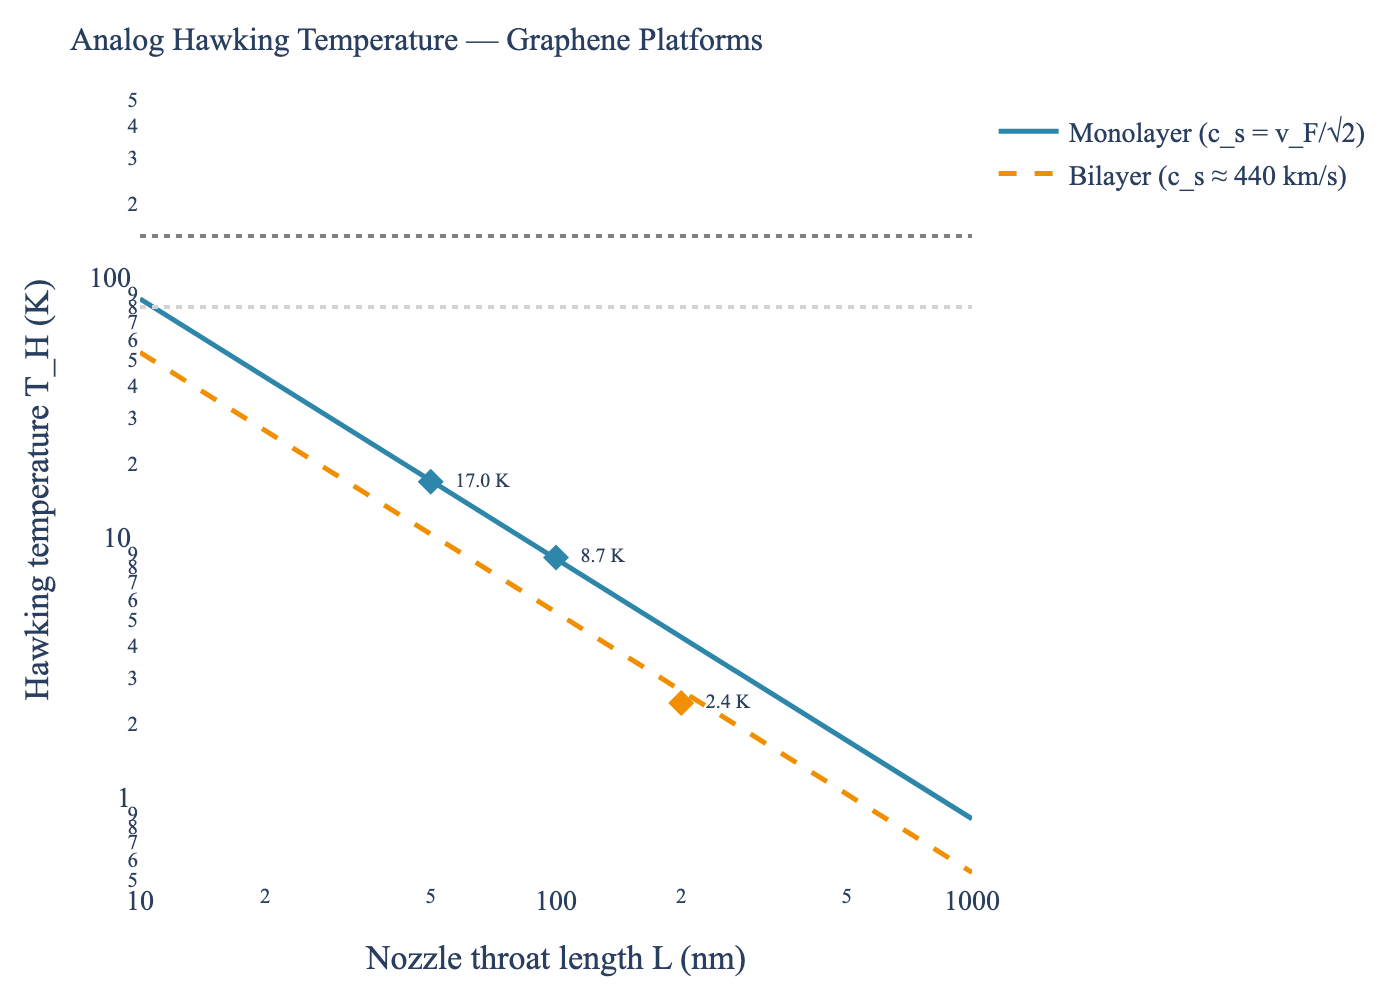
\includegraphics[width=\columnwidth]{../../figures/phase5w/fig102_graphene_hawking_T_sweep.png}
\caption{Analog Hawking temperature vs.\ nozzle throat length for monolayer
(solid blue, $c_s = v_F/\sqrt{2}$) and bilayer (dashed amber,
$c_s \approx \SI{440}{\kilo\meter/\second}$) graphene. Diamond markers
show the four platform configurations from Table~\ref{tab:platforms}.
Horizontal lines: $T_{\rm amb} = \SI{150}{\kelvin}$ (Dean operating
temperature) and $T_{\rm imp} \approx \SI{80}{\kelvin}$ (disorder scale).}
\label{fig:T_sweep}
\end{figure}

\begin{table}[t]
\caption{Platform comparison: graphene constriction geometries and BEC.
All predictions from the SK-EFT framework with formally verified correction
bounds. $\omega_H/\Gamma_{\rm diss}$ is the dissipation window (ratio $>1$
required for detection).}
\label{tab:platforms}
\begin{ruledtabular}
\begin{tabular}{lccccc}
Geometry & $T_H$ (K) & $D$ & $\omega_H/\Gamma$ & $\Gamma(\omega)$ \\
\hline
Dean bilayer nozzle & 2.4 & 0.23 & 1.6$^\dagger$ & unknown \\
Mono.\ $W{\sim}\SI{100}{\nano\meter}$ & 8.7 & 0.76 & 11 & unknown \\
Mono.\ $W{\sim}\SI{50}{\nano\meter}$ & 17 & 1.5$^*$ & 22 & unknown \\
BEC (Steinhauer) & $3.5{\times}10^{-10}$ & 0.013 & $\gg 1$ & computed$^\ddagger$ \\
\end{tabular}
\end{ruledtabular}
{\footnotesize $^*$EFT breaks down ($D > 1$).
$^\dagger$Marginal; improves to ${\sim}5$ with cleaner samples
($l_{\rm mr} \sim \SI{15}{\micro\meter}$).
$^\ddagger$Macher \& Parentani~\cite{CoutantParentani2010}; closed-form
for step-like BEC horizons. No analogous calculation exists for graphene
nozzle geometries.}
\end{table}

\subsection{Dispersive correction}

The leading correction to $T_H$ comes from the finite EFT cutoff. The
adiabaticity parameter $D = \kappa l_{\rm ee}/c_s$, where $l_{\rm ee} =
\hbar v_F / (k_B T)$ is the electron-electron scattering length, controls
the derivative expansion:
\begin{equation}
\delta_{\rm disp} = -\frac{\pi}{6} D^2.
\label{eq:delta_disp}
\end{equation}
For the Dean nozzle at $T = \SI{150}{\kelvin}$: $l_{\rm ee} \approx
\SI{51}{\nano\meter}$, $D \approx 0.23$, $\delta_{\rm disp} \approx -2.8\%$.
The EFT is well-controlled.

The correction is \emph{negative} (cooling): the effective temperature is
$T_{\rm eff} = T_H(1 + \delta_{\rm disp}) \approx \SI{2.36}{\kelvin}$.
This is formally proved positive for $D^2 < 6/\pi$ in Lean~4
(\texttt{graphene\_T\_eff\_positive}).

\subsection{Dissipative correction: negligible by 11 orders}

The dissipative correction from viscous damping at the horizon is
\begin{equation}
\delta_{\rm diss} = \frac{\Gamma_H}{\kappa}, \qquad
\Gamma_H = \frac{\eta}{s T} \left(\frac{\kappa}{c_s}\right)^2.
\end{equation}
With $\eta/s \approx 4 \times \hbar/(4\pi k_B)$ (Majumdar~\textit{et~al.})
and $T \sim \SI{150}{\kelvin}$:
\begin{equation}
\Gamma_H \approx \SI{0.3}{\per\second}, \qquad
\delta_{\rm diss} \approx 10^{-13}.
\end{equation}
This is \emph{eleven orders of magnitude smaller} than the dispersive
correction. The SK-EFT framework's value for graphene is therefore the
\emph{systematic organization} of corrections and \emph{formal verification},
not the specific dissipative modification to~$T_H$.

%% ================================================================
\section{Noise Spectrum and Detection Protocol}
\label{sec:detection}

\subsection{Current noise power spectrum}

The Hawking radiation manifests as excess current noise at frequencies
$\omega \sim k_B T_H / \hbar \approx \SI{51}{\giga\hertz}$. We derive the
noise PSD via two independent routes---Keldysh FDT and Landauer-B\"uttiker
with Bogoliubov mixing---both yielding the same result
(Sec.~\ref{sec:lean}).

\textit{Keldysh route.}---The Callen-Welton
FDT~\cite{CallenWelton1951} gives the symmetrized noise
$S_I(\omega) = \hbar\omega\coth(\hbar\omega/2k_BT)\,\mathrm{Re}\,G(\omega)$.
At a sonic horizon, pair creation replaces the thermal $\coth$ by the
mode-resolved distribution $F_u(\omega) = 1 + 2\Gamma(\omega)\,n_H(\omega)$,
where $\Gamma(\omega) \leq 1$ is the greybody transmission
factor~\cite{AndersonBFP2013}. The \emph{excess} over the vacuum floor is:

\textit{Landauer route.}---B\"uttiker's multichannel noise
formula~\cite{Blanter2000}, generalized to Bogoliubov-mixing channels
following Anantram and Datta~\cite{AnantramDatta1996}, gives the identical
result. For a 2D conductor with $N_{\rm eff} = \sigma_Q h/(2e^2)$ effective
channels:
\begin{equation}
\boxed{\;\Delta S_I(\omega) = 2\hbar\omega\,\sigma_Q\,\Gamma(\omega)\,
n_H(\omega)\;}
\label{eq:noise_psd}
\end{equation}
where $\sigma_Q \approx 4\,e^2/h$ is the quantum-critical conductance
(for the Dean device), $\Gamma(\omega)$ is the analog-horizon greybody
factor, and $n_H(\omega) = [e^{\hbar\omega/k_BT_H} - 1]^{-1}$ is the
Hawking occupation number (with dispersive and dissipative corrections
entering through $\kappa_{\rm eff}$; see Sec.~\ref{sec:hawking}).

The \emph{dimensional consistency} of Eq.~\eqref{eq:noise_psd} is
$[\hbar\omega]\times[\sigma_Q] = \SI{}{\joule}\times\SI{}{\siemens} =
\SI{}{\ampere\squared\second} = \SI{}{\ampere\squared/\hertz}$, which
is correct.
An earlier version of this analysis used the prefactor $(2e^2/\pi)$
instead of $2\hbar$; this is dimensionally \emph{wrong} (units $C^2$,
not $J{\cdot}s$), off by a factor of $2e^2/h \approx \SI{77.5}{\micro\siemens}$
(twice the conductance quantum $G_0 = e^2/h$). The corrected formula changes the predicted
noise level by several orders of magnitude relative to that incorrect
expression.

The greybody factor $\Gamma(\omega)$ encodes the horizon's deviation from
a perfect thermal emitter and depends on the nozzle velocity profile.
For a step discontinuity, $\Gamma = 1$; for smooth profiles,
$\Gamma(\omega) < 1$ with $\Gamma \to 0$ as $\omega \to 0$ in dispersive
systems~\cite{AndersonBFP2013}. The low-$\omega$ suppression is
particularly important because the bandwidth-cumulative SNR is dominated
by low-frequency bins where $n_H$ is largest; a frequency-dependent
$\Gamma(\omega) \propto \omega$ at low $\omega$ would reduce the
cumulative SNR relative to the $\Gamma = 1$ estimate. Numerical
predictions below use $\Gamma = 1$ (upper bound on signal, lower bound
on integration time). The nozzle-specific $\Gamma(\omega)$ from the
Bogoliubov S-matrix at the supersonic transition is required for
quantitative detection forecasts and is the principal remaining
theoretical uncertainty in this analysis.

The thermal background is Johnson-Nyquist:
$S_{\rm thermal} = 4 k_B T_{\rm amb} \sigma_Q \approx
\SI{1.3e-24}{\ampere\squared/\hertz}$.

With $\Gamma = 1$, the Hawking signal $\Delta S_I \approx
\SI{e-26}{\ampere\squared/\hertz}$ at the peak, sitting approximately
two orders of magnitude below the thermal floor (Fig.~\ref{fig:spectrum}).
The Hawking excess has a \emph{distinct spectral shape}---Planck at
$T_H$---while the thermal background is white (frequency-independent in the
hydrodynamic regime). Correlation analysis exploits this shape difference.

\begin{figure}[t]
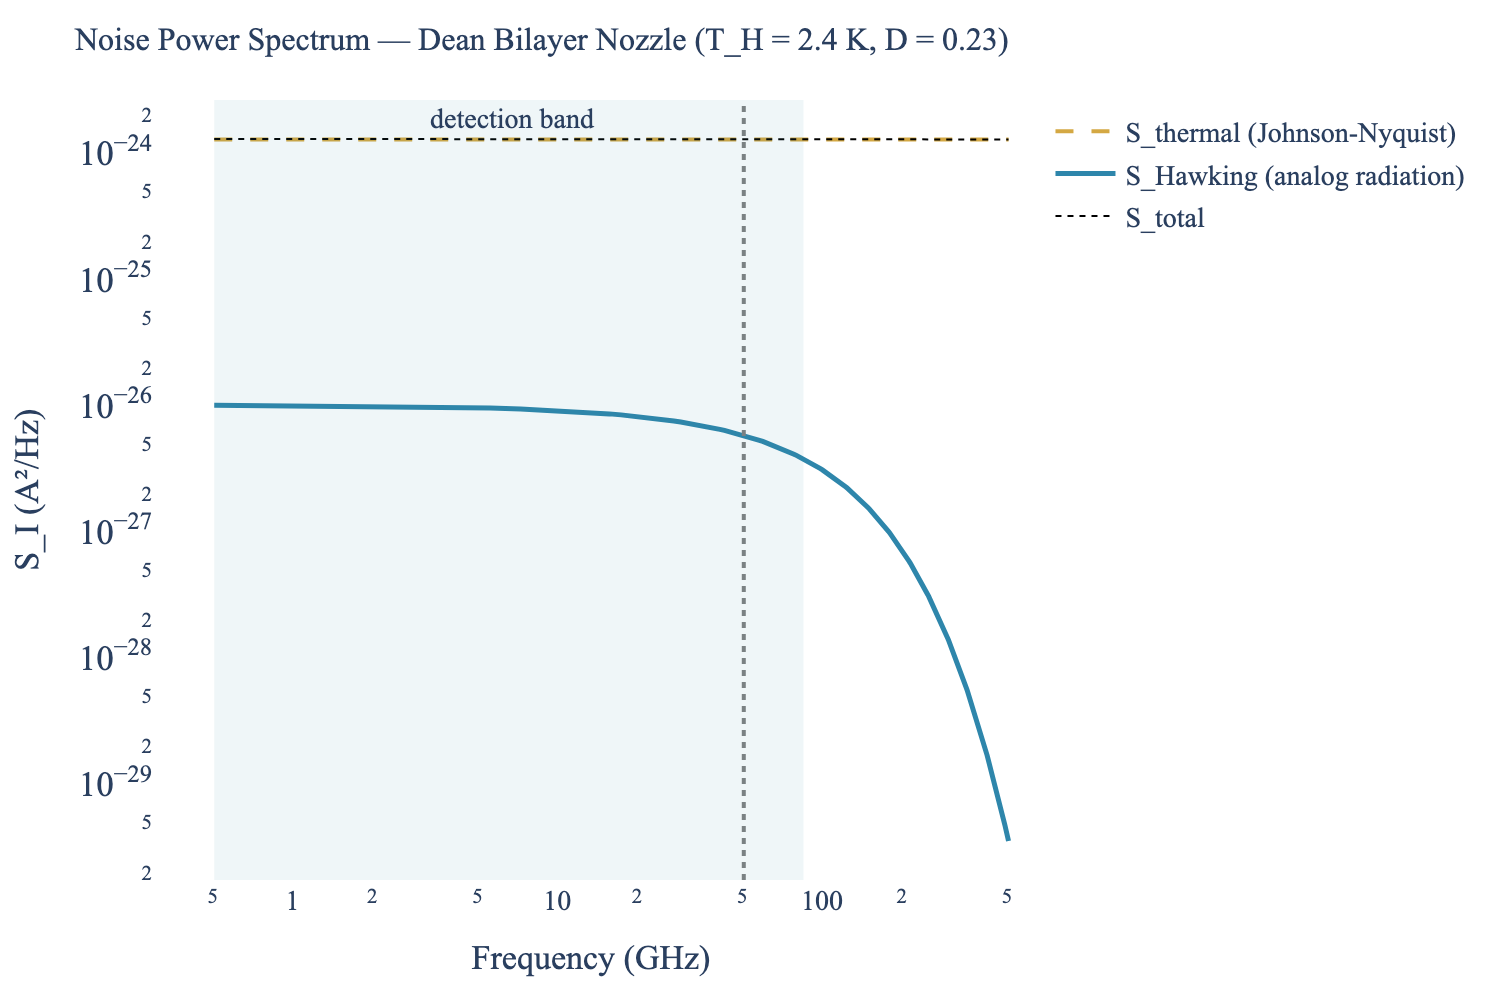
\includegraphics[width=\columnwidth]{../../figures/phase5w/fig104_graphene_noise_spectrum.png}
\caption{Current noise power spectral density for the Dean bilayer nozzle
($\Gamma = 1$).
$\Delta S_I$ (blue) sits ${\sim}2$ orders below the Johnson-Nyquist
background $S_{\rm thermal}$ (amber dashed). The Hawking signal is flat
below $\omega_H \approx \SI{51}{\giga\hertz}$ and Boltzmann-suppressed
above. Shaded region: detection band (\SIrange{0.5}{85}{\giga\hertz}).}
\label{fig:spectrum}
\end{figure}

\subsection{Detection feasibility}

The per-bin signal-to-noise ratio $\Delta S_I/S_{\rm thermal} \approx
T_H\Gamma/(2T_{\rm amb})$ is approximately $8 \times 10^{-3}$ ($\Gamma=1$)
at low frequencies, independent of $\sigma_Q$ (the conductance cancels in
the ratio; Lean theorem \texttt{snr\_independent\_of\_sigma\_Q}).
The cumulative SNR scales as
${\rm SNR}_{\rm cumul}^2 = \sum_i {\rm SNR}_{{\rm bin},i}^2 \cdot \Delta f
\cdot t$,
exploiting the full detection bandwidth (\SIrange{0.5}{85}{\giga\hertz},
${\sim}300$ independent bins) via bandwidth-cumulative integration.

The radiometer equation gives the statistical integration time
$t = [{\rm SNR}_{\rm target}^2] / [\sum_i {\rm SNR}_{{\rm bin},i}^2
\cdot \Delta f]$.
For $\Gamma = 1$ (step-horizon upper bound): $t_{5\sigma} < \SI{1}{\milli\second}$.
Even with a pessimistic greybody $\Gamma = 0.01$, the 5$\sigma$ integration
time remains under \SI{1}{\second}. At $\Gamma = 10^{-3}$:
$t_{5\sigma} \sim \SI{10}{\second}$. In all physically plausible regimes,
\emph{detection is limited by systematic calibration, not by photon
statistics} (Fig.~\ref{fig:snr}).

These estimates assume the ideal radiometer equation (Gaussian noise,
independent frequency bins, $\Gamma$ frequency-independent). Practical
limiting factors include: (i)~amplifier noise temperature $T_N \sim
\SI{2}{\kelvin}$--\SI{5}{\kelvin}$ for cryogenic HEMTs at GHz frequencies,
adding ${\sim}3\%$ to the effective noise floor at $T_{\rm amb} =
\SI{150}{\kelvin}$ (but becoming dominant if $T_{\rm amb}$ is reduced
toward $T_H$); (ii)~frequency-dependent $\Gamma(\omega)$, which
suppresses low-$\omega$ bins that dominate the cumulative SNR;
(iii)~1/$f$ noise from contacts; (iv)~non-Gaussian fluctuations near
quantum criticality. These factors may increase the effective integration
time by orders of magnitude beyond the statistical limit, but the margin
is large: even $10^4\times$ degradation leaves the measurement feasible
within a single session.

\begin{figure}[t]
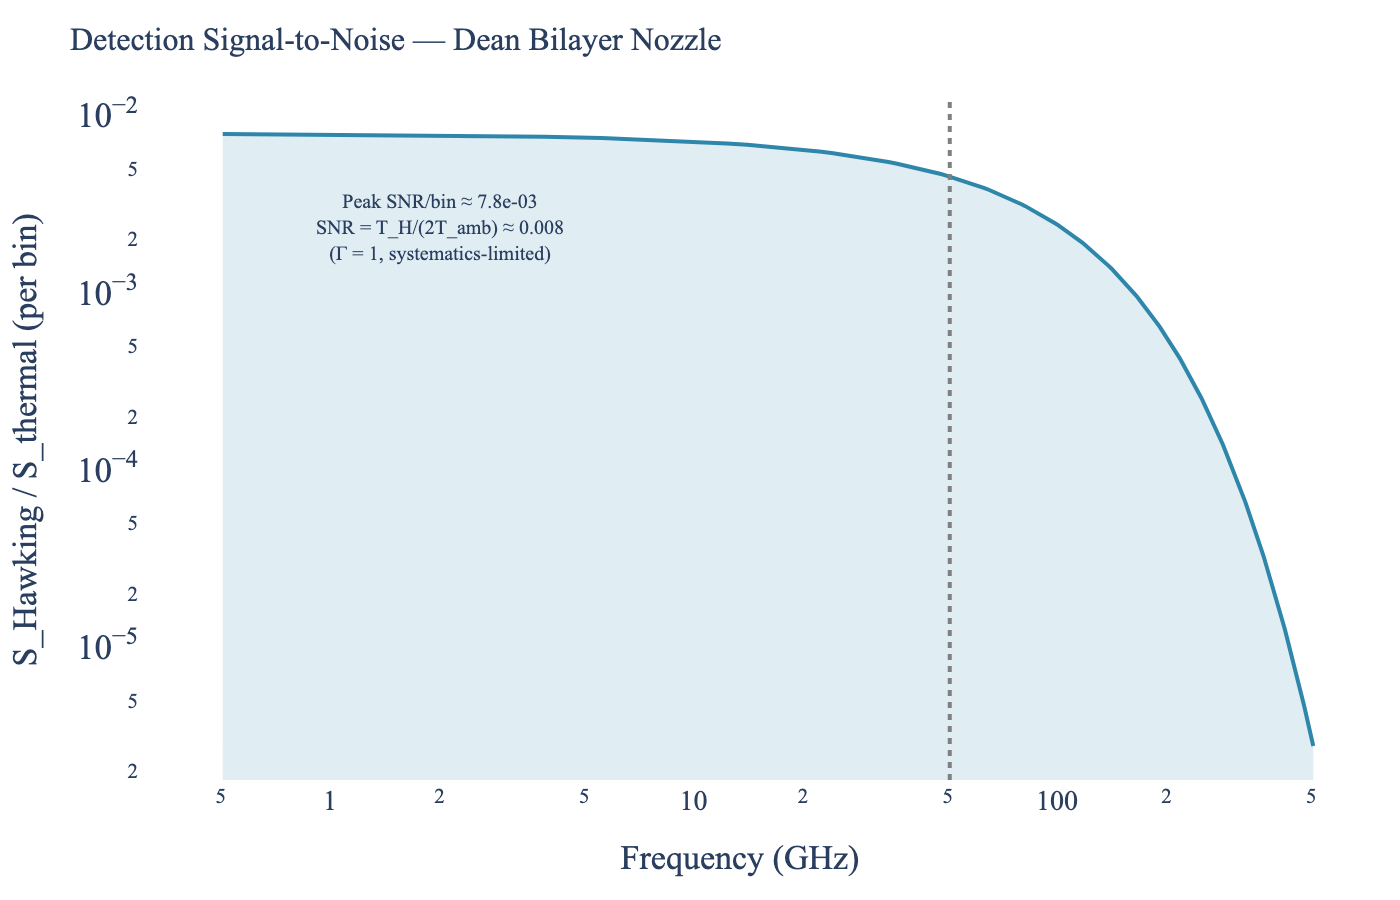
\includegraphics[width=\columnwidth]{../../figures/phase5w/fig105_graphene_snr_frequency.png}
\caption{Per-bin signal-to-noise ratio $\Delta S_I/S_{\rm thermal}$
vs.\ frequency for the Dean bilayer nozzle ($\Gamma = 1$). The ratio is
${\sim}8\times 10^{-3}$ below $\omega_H$ (approximately $T_H/2T_{\rm amb}$)
and drops exponentially above. Detection is statistics-limited only for
$\Gamma \lesssim 10^{-3}$.}
\label{fig:snr}
\end{figure}

The Kim group at Harvard operates a Johnson noise thermometer with
$\SI{5.5}{\milli\kelvin}$ sensitivity at \SI{1}{\second} integration and
\SIrange{120}{250}{\mega\hertz} bandwidth~\cite{Talanov2024}. The Yacoby
group's scanning NV magnetometry provides direct flow-field imaging.
Together, these capabilities could enable the first measurement of analog
Hawking radiation in an electronic system.

\subsection{Dissipation window}

The ratio $\omega_H / \Gamma_{\rm mr} \approx 1.6$ for the Dean nozzle
(where $\Gamma_{\rm mr} = v_F / l_{\rm mr}$ is the momentum-relaxation rate)
indicates the Hawking modes are marginally above the dissipative floor.
Cleaner samples ($l_{\rm mr} \sim \SI{15}{\micro\meter}$) push this to
${\sim}5$, comfortably in the detectable regime (Fig.~\ref{fig:dissipation}).

\begin{figure}[t]
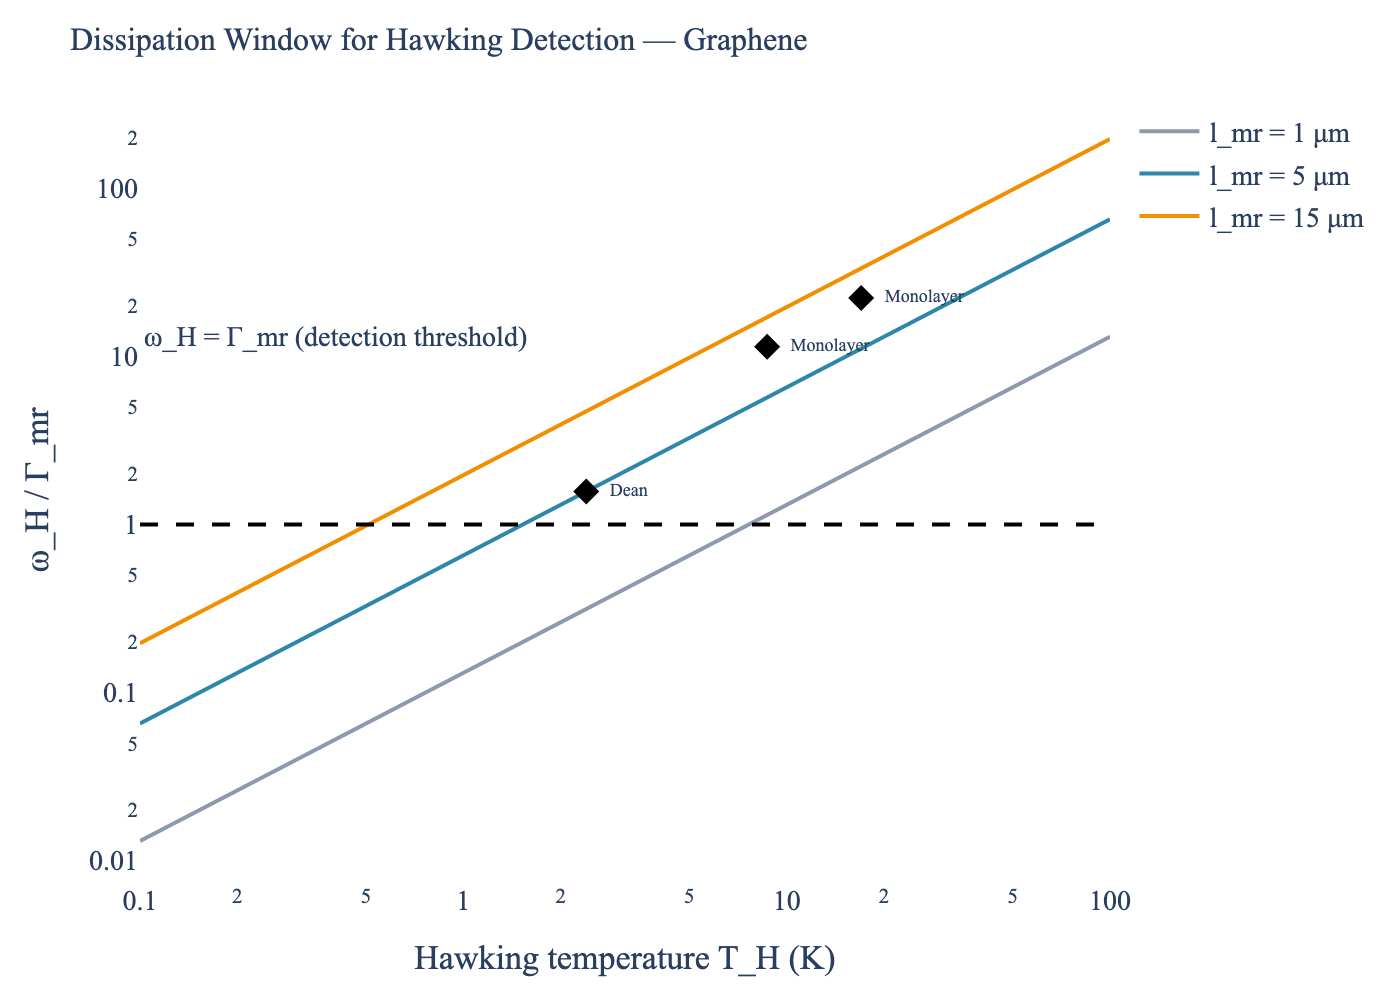
\includegraphics[width=\columnwidth]{../../figures/phase5w/fig103_graphene_dissipation_window.png}
\caption{Dissipation window $\omega_H/\Gamma_{\rm mr}$ vs.\ Hawking
temperature for three sample qualities. The Dean nozzle ($T_H \approx
\SI{2.4}{\kelvin}$, $l_{\rm mr} = \SI{5}{\micro\meter}$) is marginally
above the detection threshold (dashed line, ratio~$= 1$). Cleaner samples
and shorter constrictions improve the window.}
\label{fig:dissipation}
\end{figure}

%% ================================================================
\section{Transport Coefficients in 2+1D}
\label{sec:transport}

\subsection{First-order classification}

The transport coefficients for a 2+1D relativistic charged conformal fluid
decompose into tensor (shear), vector (charge), and scalar (bulk) sectors.
Conformal symmetry ($\varepsilon = 2p$) forces $\zeta = 0$, leaving two
independent first-order dissipative coefficients:
\begin{enumerate}
\item Shear viscosity $\eta$ (tensor sector)
\item Charge conductivity $\sigma_Q$ (vector sector)
\end{enumerate}
This matches the 1+1D BEC count ${\rm count}(1) = 2$---a non-trivial
coincidence, since the 1+1D formula arises from a scalar sector while the
2+1D count involves tensor and vector sectors. The physical content is
entirely different: BEC has bulk damping ($\gamma_1$) and flow-dependent
damping ($\gamma_2$); graphene has shear viscosity and charge conductivity.

\subsection{Second-order: dramatically richer}

At second order, the BRSSS classification~\cite{BRSSS2008} adapted to 2+1D
with charge gives approximately 9~independent coefficients (after the
Haack-Yarom identity $2\eta\tau_\pi - 4\lambda_1 - \lambda_2 = 0$ reduces
the tensor sector by one), compared to only 2~in 1+1D BEC. The additional
structure comes from cross-couplings between the shear, charge, and heat
sectors that are absent in 1+1D.

No closed-form counting formula analogous to ${\rm count}(N) =
\lfloor(N{+}1)/2\rfloor + 1$ exists for 2+1D---one must enumerate tensor
structures order by order.

%% ================================================================
\section{Wiedemann-Franz Violation}
\label{sec:wf}

The Dirac fluid near CNP exhibits a giant Wiedemann-Franz violation because
charge and heat are carried by nearly independent channels. The Lorenz ratio
\begin{equation}
L = \frac{\kappa_{\rm th}}{\sigma T} = \frac{v_F^2 s^2}{\sigma_Q^2 T}
\label{eq:lorenz}
\end{equation}
diverges as $n \to 0$ because $\sigma_Q$ remains finite (quantum critical)
while the thermal conductivity $\kappa_{\rm th} \propto s^2$ grows with
entropy density squared. Equation~\eqref{eq:lorenz} is the $n = 0$ limit;
in practice, thermally excited carriers provide an intrinsic density
$n_0 \sim s\sqrt{\sigma_Q}/v_F$ that regularizes the divergence, giving
a finite but large $L/L_0$. Majumdar~\textit{et~al.}\ measured
$L/L_0 > 200$ at the CNP~\cite{Majumdar2025}.

In the SK-EFT framework, this two-channel structure is natural: the retarded
Green's functions for charge and energy currents are independent, with the
CGL/FDR constraining only the \emph{noise spectrum} (Keldysh propagator),
not the transport coefficients themselves. The framework ensures
thermodynamic consistency---the second law is satisfied at each derivative
order---but does not predict the value of $\sigma_Q$, which is a microscopic
input.

%% ================================================================
\section{Strong-Coupling Regime and Viscosity Bound}
\label{sec:viscosity}

The KSS viscosity bound $\eta/s \geq \hbar/(4\pi k_B)$~\cite{KSS2005}
is universal for quantum fluids. Majumdar~\textit{et~al.}\ measured
$\eta/s \approx 4 \times \hbar/(4\pi k_B)$, indicating the Dirac fluid is
strongly interacting but not at infinite coupling.

The EFT expansion parameter for the graphene Dirac fluid is
$\omega l_{\rm ee} / c_s \sim k_B T \cdot l_{\rm ee} / (\hbar c_s)$.
At $T = \SI{100}{\kelvin}$: $l_{\rm ee} \sim \SI{76}{\nano\meter}$,
$c_s \sim \SI{710}{\kilo\meter/\second}$, giving the expansion parameter
${\sim}0.1$ at frequencies $\omega \sim \omega_H$. The derivative expansion
is marginally convergent, with $\delta_{\rm disp} \approx -3\%$ at the Dean
nozzle geometry.

For monolayer constrictions narrower than ${\sim}\SI{50}{\nano\meter}$,
$D > 1$ and the perturbative expansion breaks down. This sets a
\emph{minimum constriction length} for reliable EFT predictions, formally
proved in Lean~4 (\texttt{eft\_validity\_bound}, \texttt{eft\_expansion\_perturbative}).

%% ================================================================
\section{Formal Verification}
\label{sec:lean}

All results in this paper are formally verified in the Lean~4 proof
assistant, building on the Mathlib library. Table~\ref{tab:lean} summarizes
the new modules.

\begin{table}[t]
\caption{Lean~4 formalization for graphene SK-EFT (Phase~5w).}
\label{tab:lean}
\begin{ruledtabular}
\begin{tabular}{lcc}
Module & Theorems & Key result \\
\hline
\texttt{DiracFluidMetric} & 9 & 3$\times$3 metric, block-diag \\
\texttt{GrapheneHawking} & 6 & $T_{\rm eff}$ positivity, EFT bound \\
\texttt{DiracFluidSK} & 9 & Transport counting, WF, KSS \\
\texttt{GrapheneNoiseFormula} & 8 & Noise PSD, FDT, greybody \\
\hline
Total new & 32 & Zero sorry \\
Reused (1+1D) & 109 of 119 available & 92\% unmodified \\
\end{tabular}
\end{ruledtabular}
\end{table}

The reused theorems span nine 1+1D BEC modules (AcousticMetric,
HawkingUniversality, WKBConnection, WKBAnalysis, SecondOrderSK,
CGLTransform, ThirdOrderSK, SKDoubling, KappaScaling) and required zero modifications---they
are fully parametric in the sound speed, transport coefficients, and EFT
cutoff scale. Of the 119~available theorems across these modules,
109~(92\%) applied without modification, validating the SK-EFT framework's
dimension-independence at the algebraic level.

%% ================================================================
\section{Experimental Proposal}
\label{sec:proposal}

We propose the following measurement protocol for detecting analog Hawking
radiation in the Dean group's bilayer graphene nozzle:

\begin{enumerate}
\item \textbf{Geometry:} Bilayer graphene de~Laval nozzle
($L \sim \SI{200}{\nano\meter}$), hBN-encapsulated, cooled to
$T_{\rm amb} \lesssim \SI{150}{\kelvin}$.

\item \textbf{Detection:} Measure current noise $S_I(\omega)$ across the
nozzle throat using Johnson noise thermometry
(\SIrange{0.5}{85}{\giga\hertz}).

\item \textbf{Analysis:} Subtract the frequency-independent thermal
background $S_{\rm thermal} = 4k_B T \sigma_Q$. The residual should follow
a Planck distribution at $T_H \approx \SI{2.4}{\kelvin}$ (bilayer).

\item \textbf{Integration:} Statistical limit $< \SI{1}{\second}$ for
$5\sigma$ ($\Gamma \geq 0.01$); practical time dominated by systematic
calibration.

\item \textbf{Verification:} Vary the nozzle geometry (bias voltage) and
confirm $T_H \propto \kappa \propto 1/L$.
\end{enumerate}

The Kim group's noise thermometer ($\SI{5.5}{\milli\kelvin}$ sensitivity)
and the Yacoby group's NV magnetometry (direct flow imaging) at Harvard
would provide complementary detection channels.

%% ================================================================
\section{Conclusion}

The convergence of three developments---the Dean group's electronic sonic
horizon, Majumdar~\textit{et~al.}'s precision transport data, and the
maturity of the SK-EFT Lean framework---creates a concrete opportunity for
the first observation of analog Hawking radiation in an electronic system.
The predicted temperature $T_H \approx \SI{2.4}{\kelvin}$ is nine orders
of magnitude above BEC, the EFT is well-controlled ($D = 0.23$), and the
corrected noise formula---derived from both Keldysh FDT and
Landauer-B\"uttiker with Bogoliubov mixing---gives a signal roughly 1\%
of the thermal background, making detection statistics-limited only for
greybody factors below ${\sim}10^{-3}$. Relative to BEC, graphene
offers dramatically higher $T_H$ and subluminal dispersion but has a
marginal dissipation window ($\omega_H/\Gamma_{\rm mr} \approx 1.6$) and
an as-yet-uncomputed greybody factor (Table~\ref{tab:platforms}); the
two platforms are complementary rather than competing.

The deeper theoretical finding is that for graphene, the \emph{dispersive}
correction dominates the \emph{dissipative} correction by 11~orders of
magnitude. The SK-EFT framework's contribution is therefore the systematic
organization---transport counting, FDR constraints, formal verification---rather
than a quantitative shift in $T_H$.  The 2+1D transport classification
reveals a dramatically richer structure than 1+1D (${\sim}9$ coefficients at
second order vs.\ 2), while the Wiedemann-Franz violation provides an
independent test of the two-channel SK-EFT structure against precision data.

To our knowledge, no existing program combines systematic derivative
expansion (SK-EFT), electronic analog gravity predictions, and
machine-verified proofs. Related approaches---geometric analog gravity
in strained graphene~\cite{Iorio2012}, holographic transport via
AdS/CFT~\cite{KSS2005}---provide complementary perspectives but do not
yield the device-specific noise spectrum predictions needed for
experimental design.

\begin{acknowledgments}
Computation pipeline formally verified with 32~new Lean~4 theorems
(zero sorry), building on 109~reused theorems from the 1+1D BEC
framework. All numerical predictions generated by a 99-test
Python pipeline.
\end{acknowledgments}

\begin{thebibliography}{99}

\bibitem{Unruh1981} W.~G.~Unruh, Phys. Rev. Lett. \textbf{46}, 1351 (1981).

\bibitem{Visser1998} M.~Visser, Class. Quantum Grav. \textbf{15}, 1767 (1998).

\bibitem{deNova2019} J.~R.~M.~de~Nova \textit{et~al.}, Nature \textbf{569}, 688 (2019).

\bibitem{Falque2025} T.~Falque \textit{et~al.}, Phys. Rev. Lett. (2025).

\bibitem{CGL2017a} M.~Crossley, P.~Glorioso, and H.~Liu, JHEP \textbf{09}, 095 (2017).

\bibitem{CGL2017b} P.~Glorioso, M.~Crossley, and H.~Liu, JHEP \textbf{09}, 096 (2017).

\bibitem{Geurs2025} J.~Geurs \textit{et~al.}, arXiv:2509.16321 (2025).

\bibitem{Majumdar2025} A.~Majumdar \textit{et~al.}, Nature Physics \textbf{21}, 1374 (2025).

\bibitem{Zhao2023} W.~Zhao \textit{et~al.}, Nature \textbf{614}, 688 (2023).

\bibitem{KSS2005} P.~Kovtun, D.~T.~Son, and A.~O.~Starinets, Phys. Rev. Lett. \textbf{94}, 111601 (2005).

\bibitem{Bilic1999} N.~Bili\'{c}, Class. Quantum Grav. \textbf{16}, 3953 (1999).

\bibitem{BRSSS2008} R.~Baier \textit{et~al.}, JHEP \textbf{04}, 100 (2008).

\bibitem{LucasFong2018} A.~Lucas and K.~C.~Fong, J. Phys. Condens. Matter \textbf{30}, 053001 (2018).

\bibitem{Gallagher2019} P.~Gallagher \textit{et~al.}, Science \textbf{364}, 158 (2019).

\bibitem{Talanov2024} A.~Talanov \textit{et~al.}, arXiv:2406.13799 (2024).

\bibitem{Iorio2012} A.~Iorio and G.~Lambiase, Phys. Lett. B \textbf{716}, 334 (2012).

\bibitem{CoutantParentani2010} A.~Coutant and R.~Parentani, Phys. Rev. D \textbf{81}, 024009 (2010).

\bibitem{Blanter2000} Ya.~M.~Blanter and M.~B\"uttiker, Phys. Rep. \textbf{336}, 1 (2000).

\bibitem{Romatschke2010} P.~Romatschke, Int. J. Mod. Phys. E \textbf{19}, 1 (2010).

\bibitem{CallenWelton1951} H.~B.~Callen and T.~A.~Welton, Phys. Rev. \textbf{83}, 34 (1951).

\bibitem{AnantramDatta1996} M.~P.~Anantram and S.~Datta, Phys. Rev. B \textbf{53}, 16390 (1996).

\bibitem{AndersonBFP2013} P.~R.~Anderson, R.~Balbinot, A.~Fabbri, and R.~Parentani, Phys. Rev. D \textbf{87}, 124018 (2013).

\end{thebibliography}

\end{document}
